\documentclass[10pt]{article}

\usepackage{graphicx}			% Use this package to include images
\usepackage{amsmath}			% A library of many standard math expressions
\usepackage{amsfonts}
\usepackage[margin=1in]{geometry}% Sets 1in margins.
\usepackage{fancyhdr}			% Creates headers and footers
\usepackage{enumerate}          %These two package give custom labels to a list
\usepackage[shortlabels]{enumitem}
\usepackage{braket}
\usepackage{physics}
\usepackage{pgfplots}
\usepackage{tikz}
\usepackage{xcolor}
\usepackage{mathtools}
\usepackage{url}
\usepackage{listings}
\usepackage{geometry}
\usepackage{titling}

%% LISTINGS CONFIG %%

\definecolor{purple2}{RGB}{153,0,153} % there's actually no standard purple
\definecolor{green2}{RGB}{0,153,0} % a darker green

\lstset{
  language=Python,                   % the language
  basicstyle=\ttfamily\small,   % size of the fonts for the code
  frame = single,
  % Color settings to match IDLE style
  keywordstyle=\color{orange},       % core keywords
  keywordstyle={[2]\color{purple2}}, % built-ins
  stringstyle=\color{green2},%
  showstringspaces=false,
  commentstyle=\color{red},%
  upquote=true,                      % requires textcomp
  numbers=left,
  breaklines=true,
}

\setlength{\droptitle}{-6em}     % Eliminate the default vertical space

\title{\textbf{ECE469 - Introduction to ML} \\ \textit{Midterm - Part 1}}
\author{Chase A. Lotito - \textit{SIUC Undergraduate}}
\date{\today}

\begin{document} %The writing for your homework should all come after this.

\maketitle


% QUESTION 1
\textbf{Question 1.} \textit{Regression in machine learning.}

\bigskip
\textbf{Solution.}

% 1.a
\smallskip
\textit{(A)}

\smallskip
Unedited, the housing dataset contains 10 features, but eventually \textit{ocean\_proximity} will be dropped, and \textit{median\_house\_value} will be chosen as the output target; all remaining columns will be the input features for the linear model.

\begin{figure}[h]
    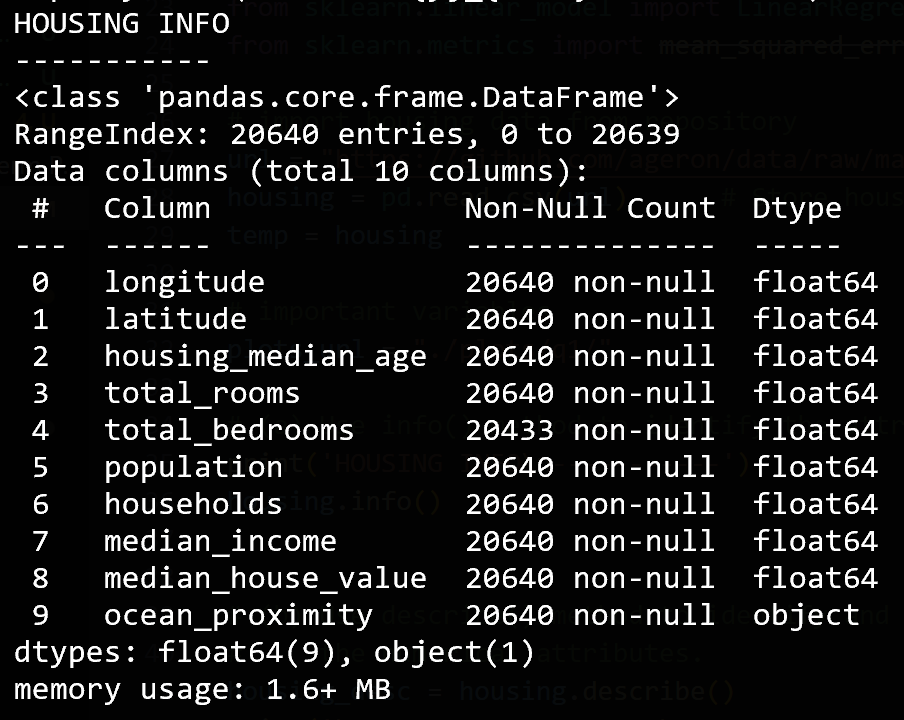
\includegraphics[width=0.6\textwidth]{../logs/housing_info.png}
    \centering
    \caption{housing.info()}
\end{figure}

% 1.b
\smallskip
\textit{(B)}
\begin{figure}[h]
    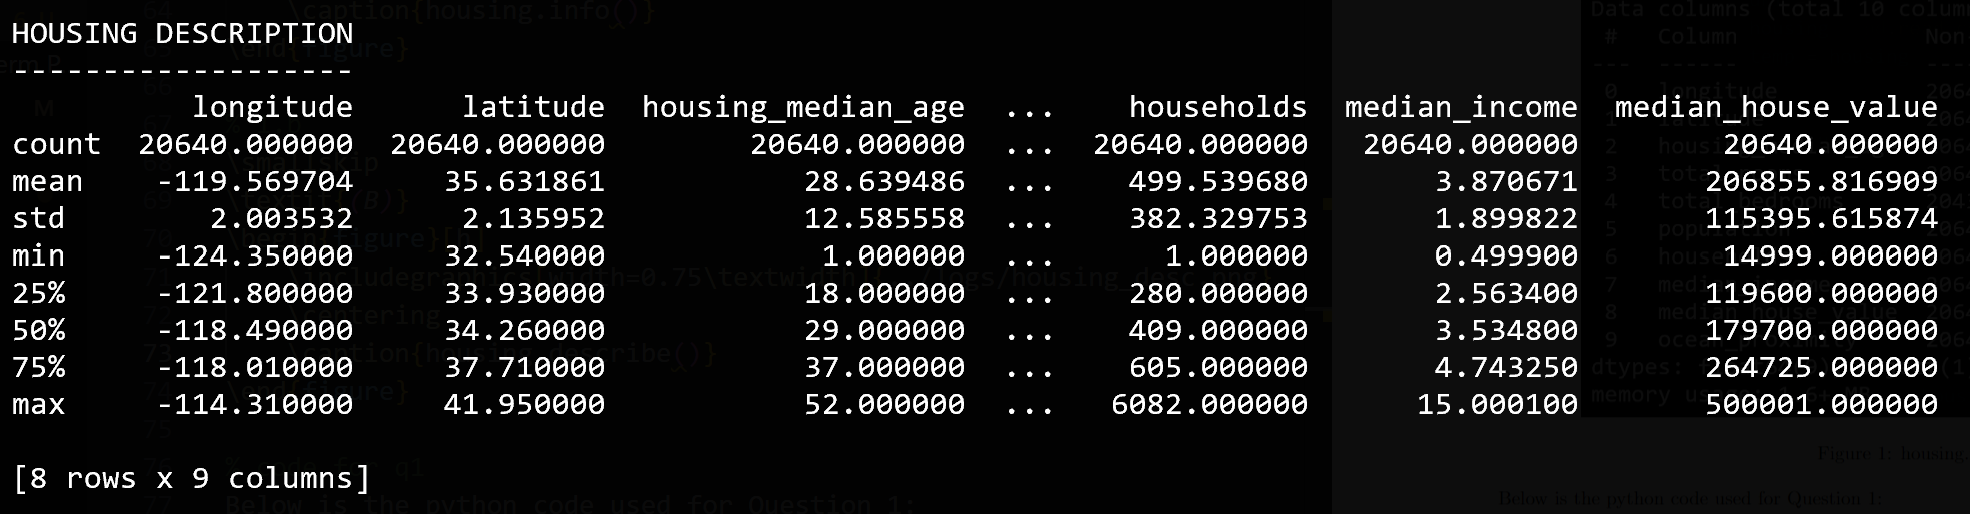
\includegraphics[width=0.85\textwidth]{../logs/housing_desc.png}
    \centering
    \caption{housing.describe()}
\end{figure}

\clearpage

% 1.c
\smallskip
\textit{(C)}
\begin{figure}[h]
    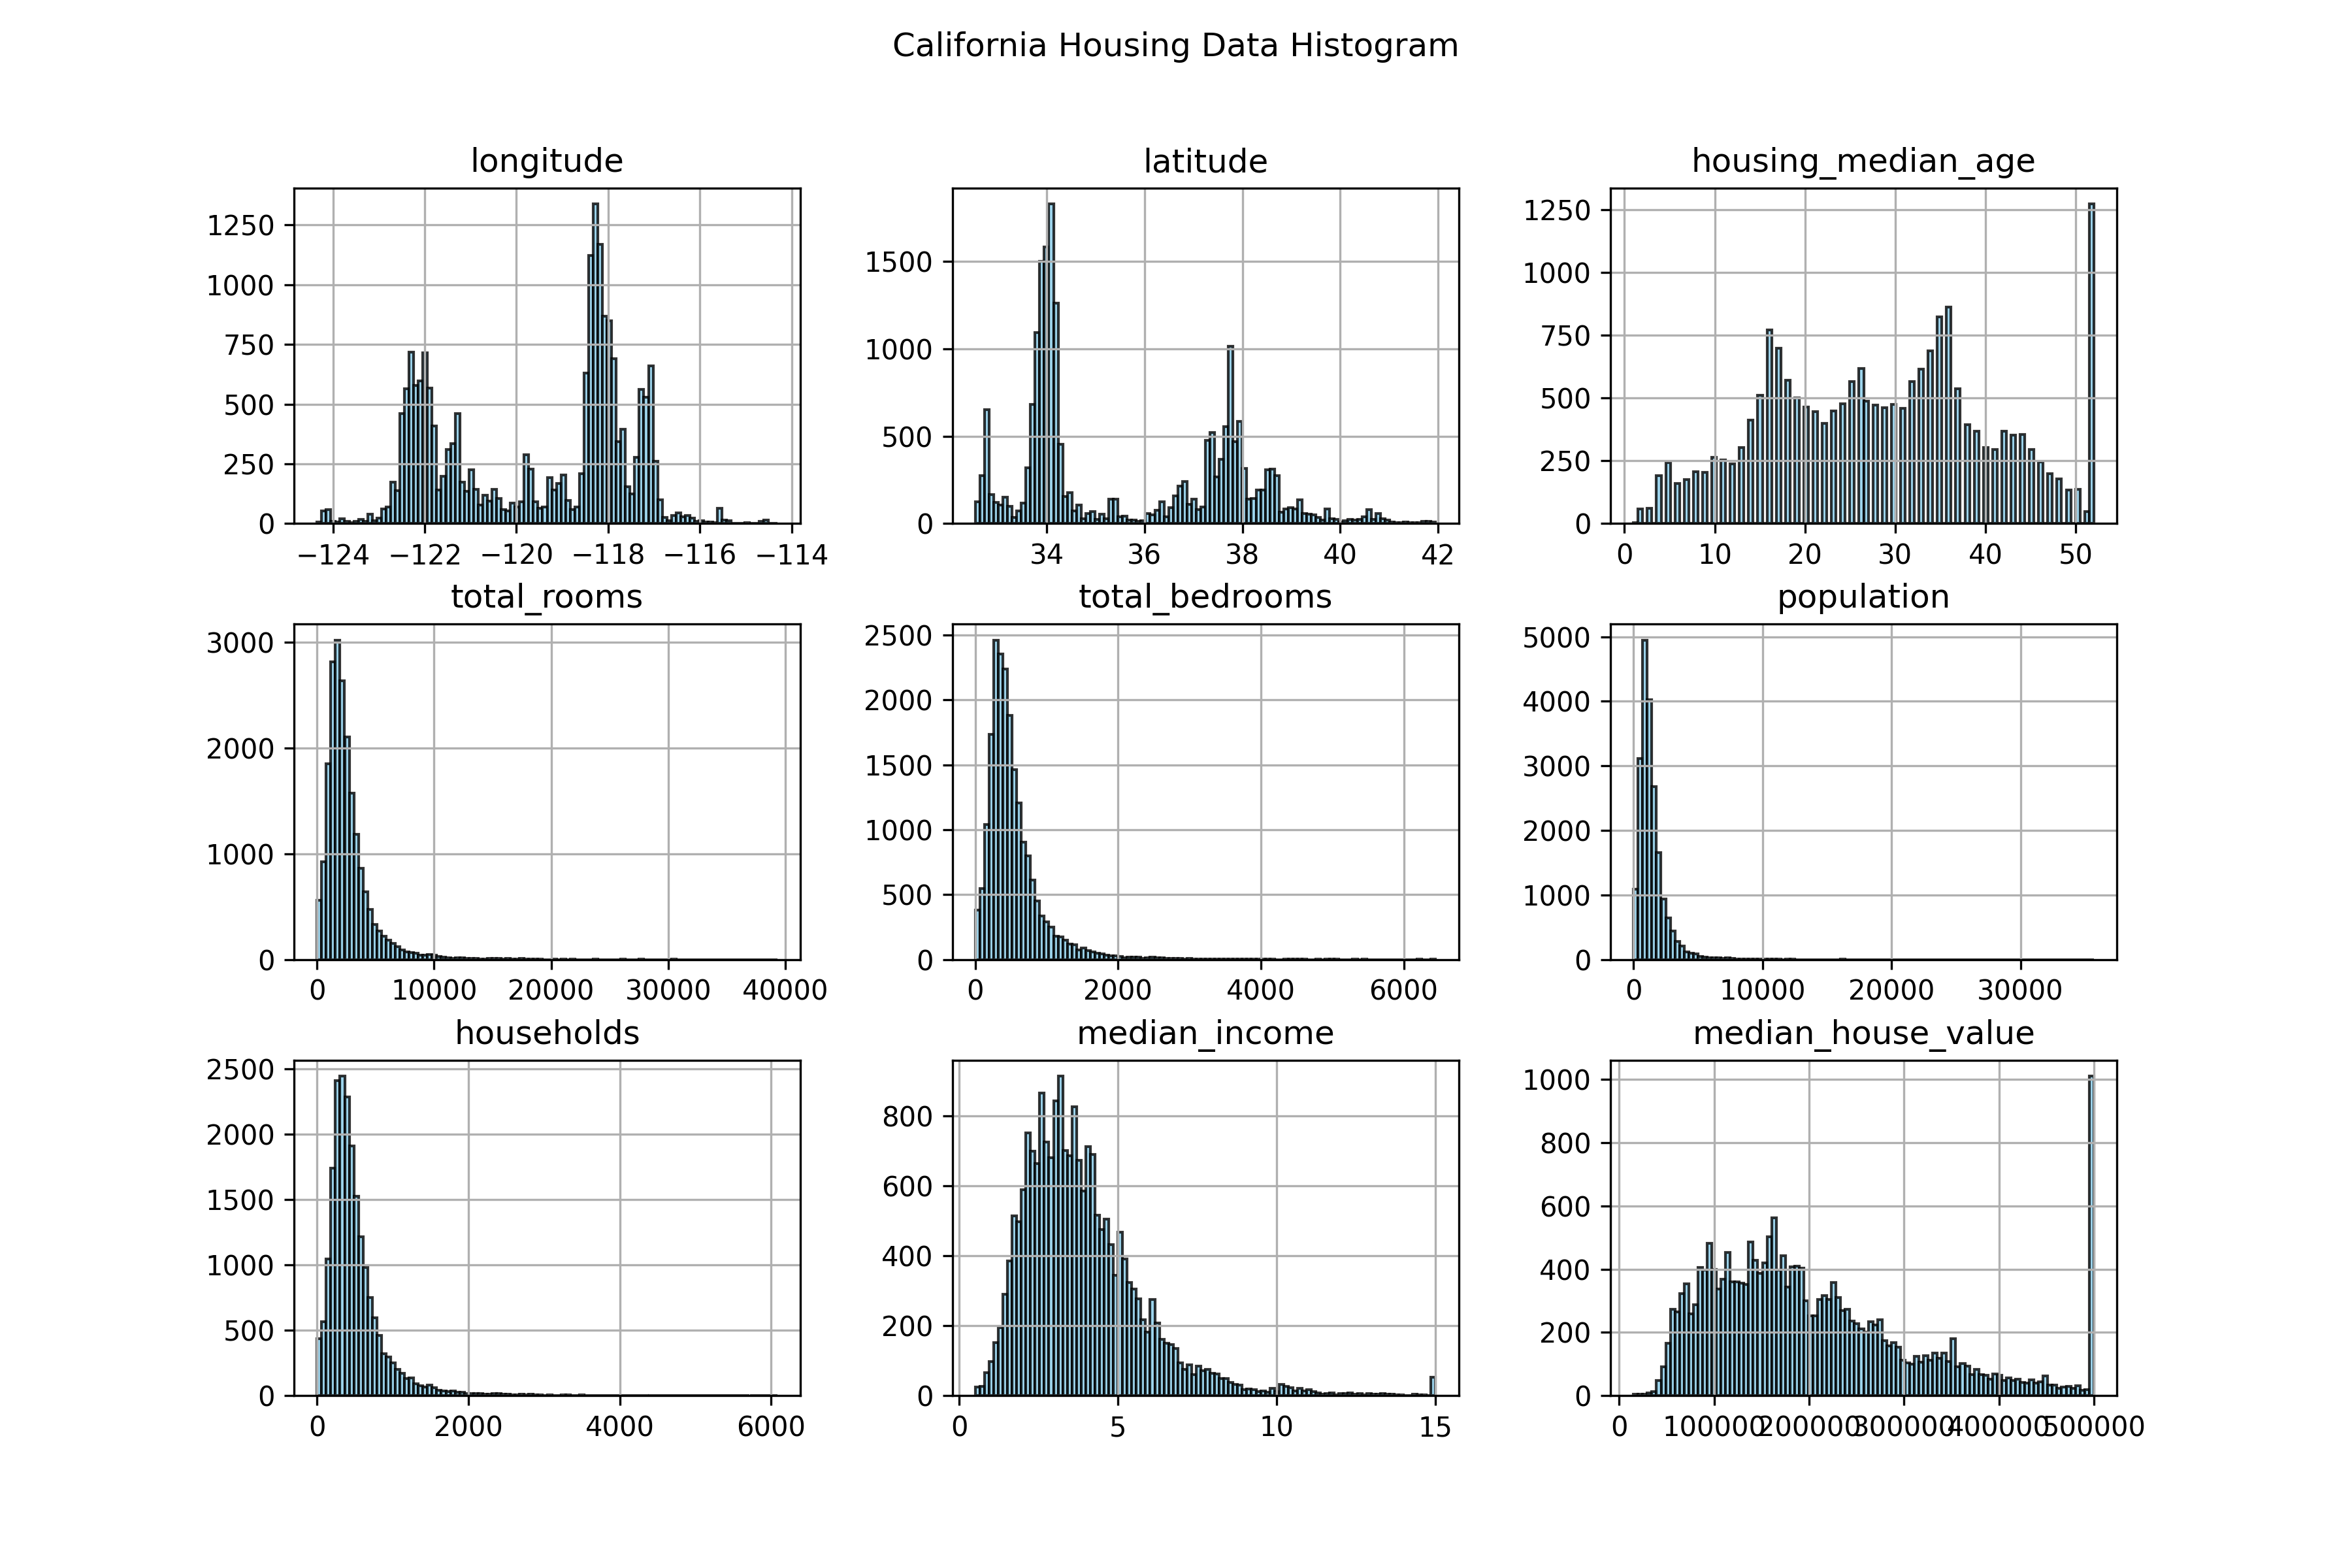
\includegraphics[width=0.95\textwidth]{../plots/q1/housing_histogram.png}
    \centering
    \caption{Housing Dataset Histogram}
\end{figure}

% 1.d
\smallskip
\textit{(D)}

\smallskip
Using \textit{SimpleImputer} from SciKit-Learn to replace missing data with the median value, and using \textit{StandardScaler} from SciKit-Learn to standardize the dataset, the dataset looks as follows:

\begin{figure}[h]
    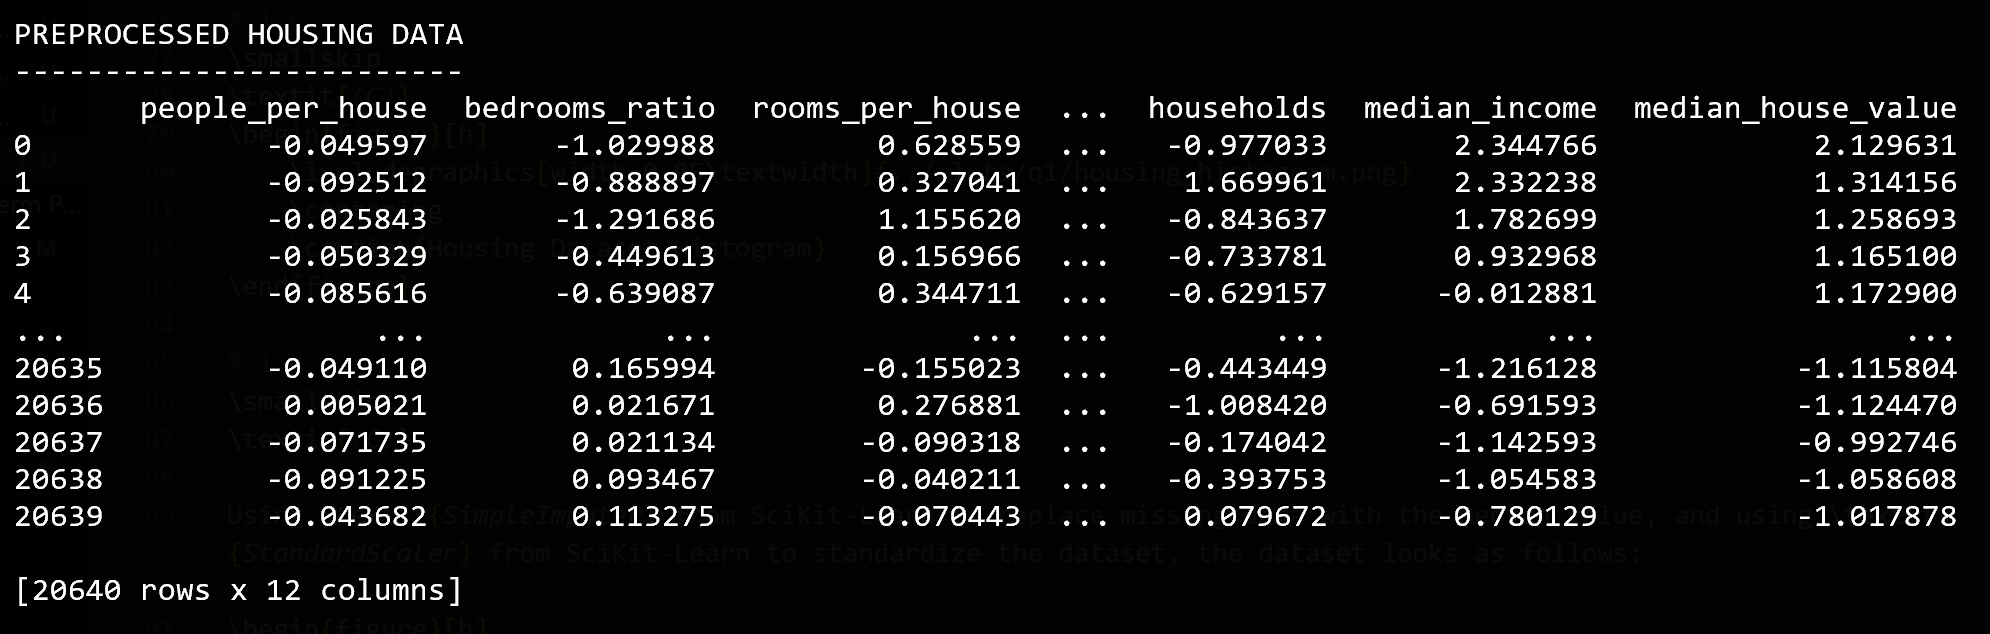
\includegraphics[width=0.85\textwidth]{../logs/housing_pre.png}
    \centering
    \caption{Preprocessed dataset}
\end{figure}

\clearpage

% 1.e
\smallskip
\textit{(E)}

\smallskip
The standardized dataset when \textit{latitude} and \textit{longitude} are plotted against each other in a scatterplot shows a 2D map of all of the houses in the housing dataset.

\begin{figure}[!h]
    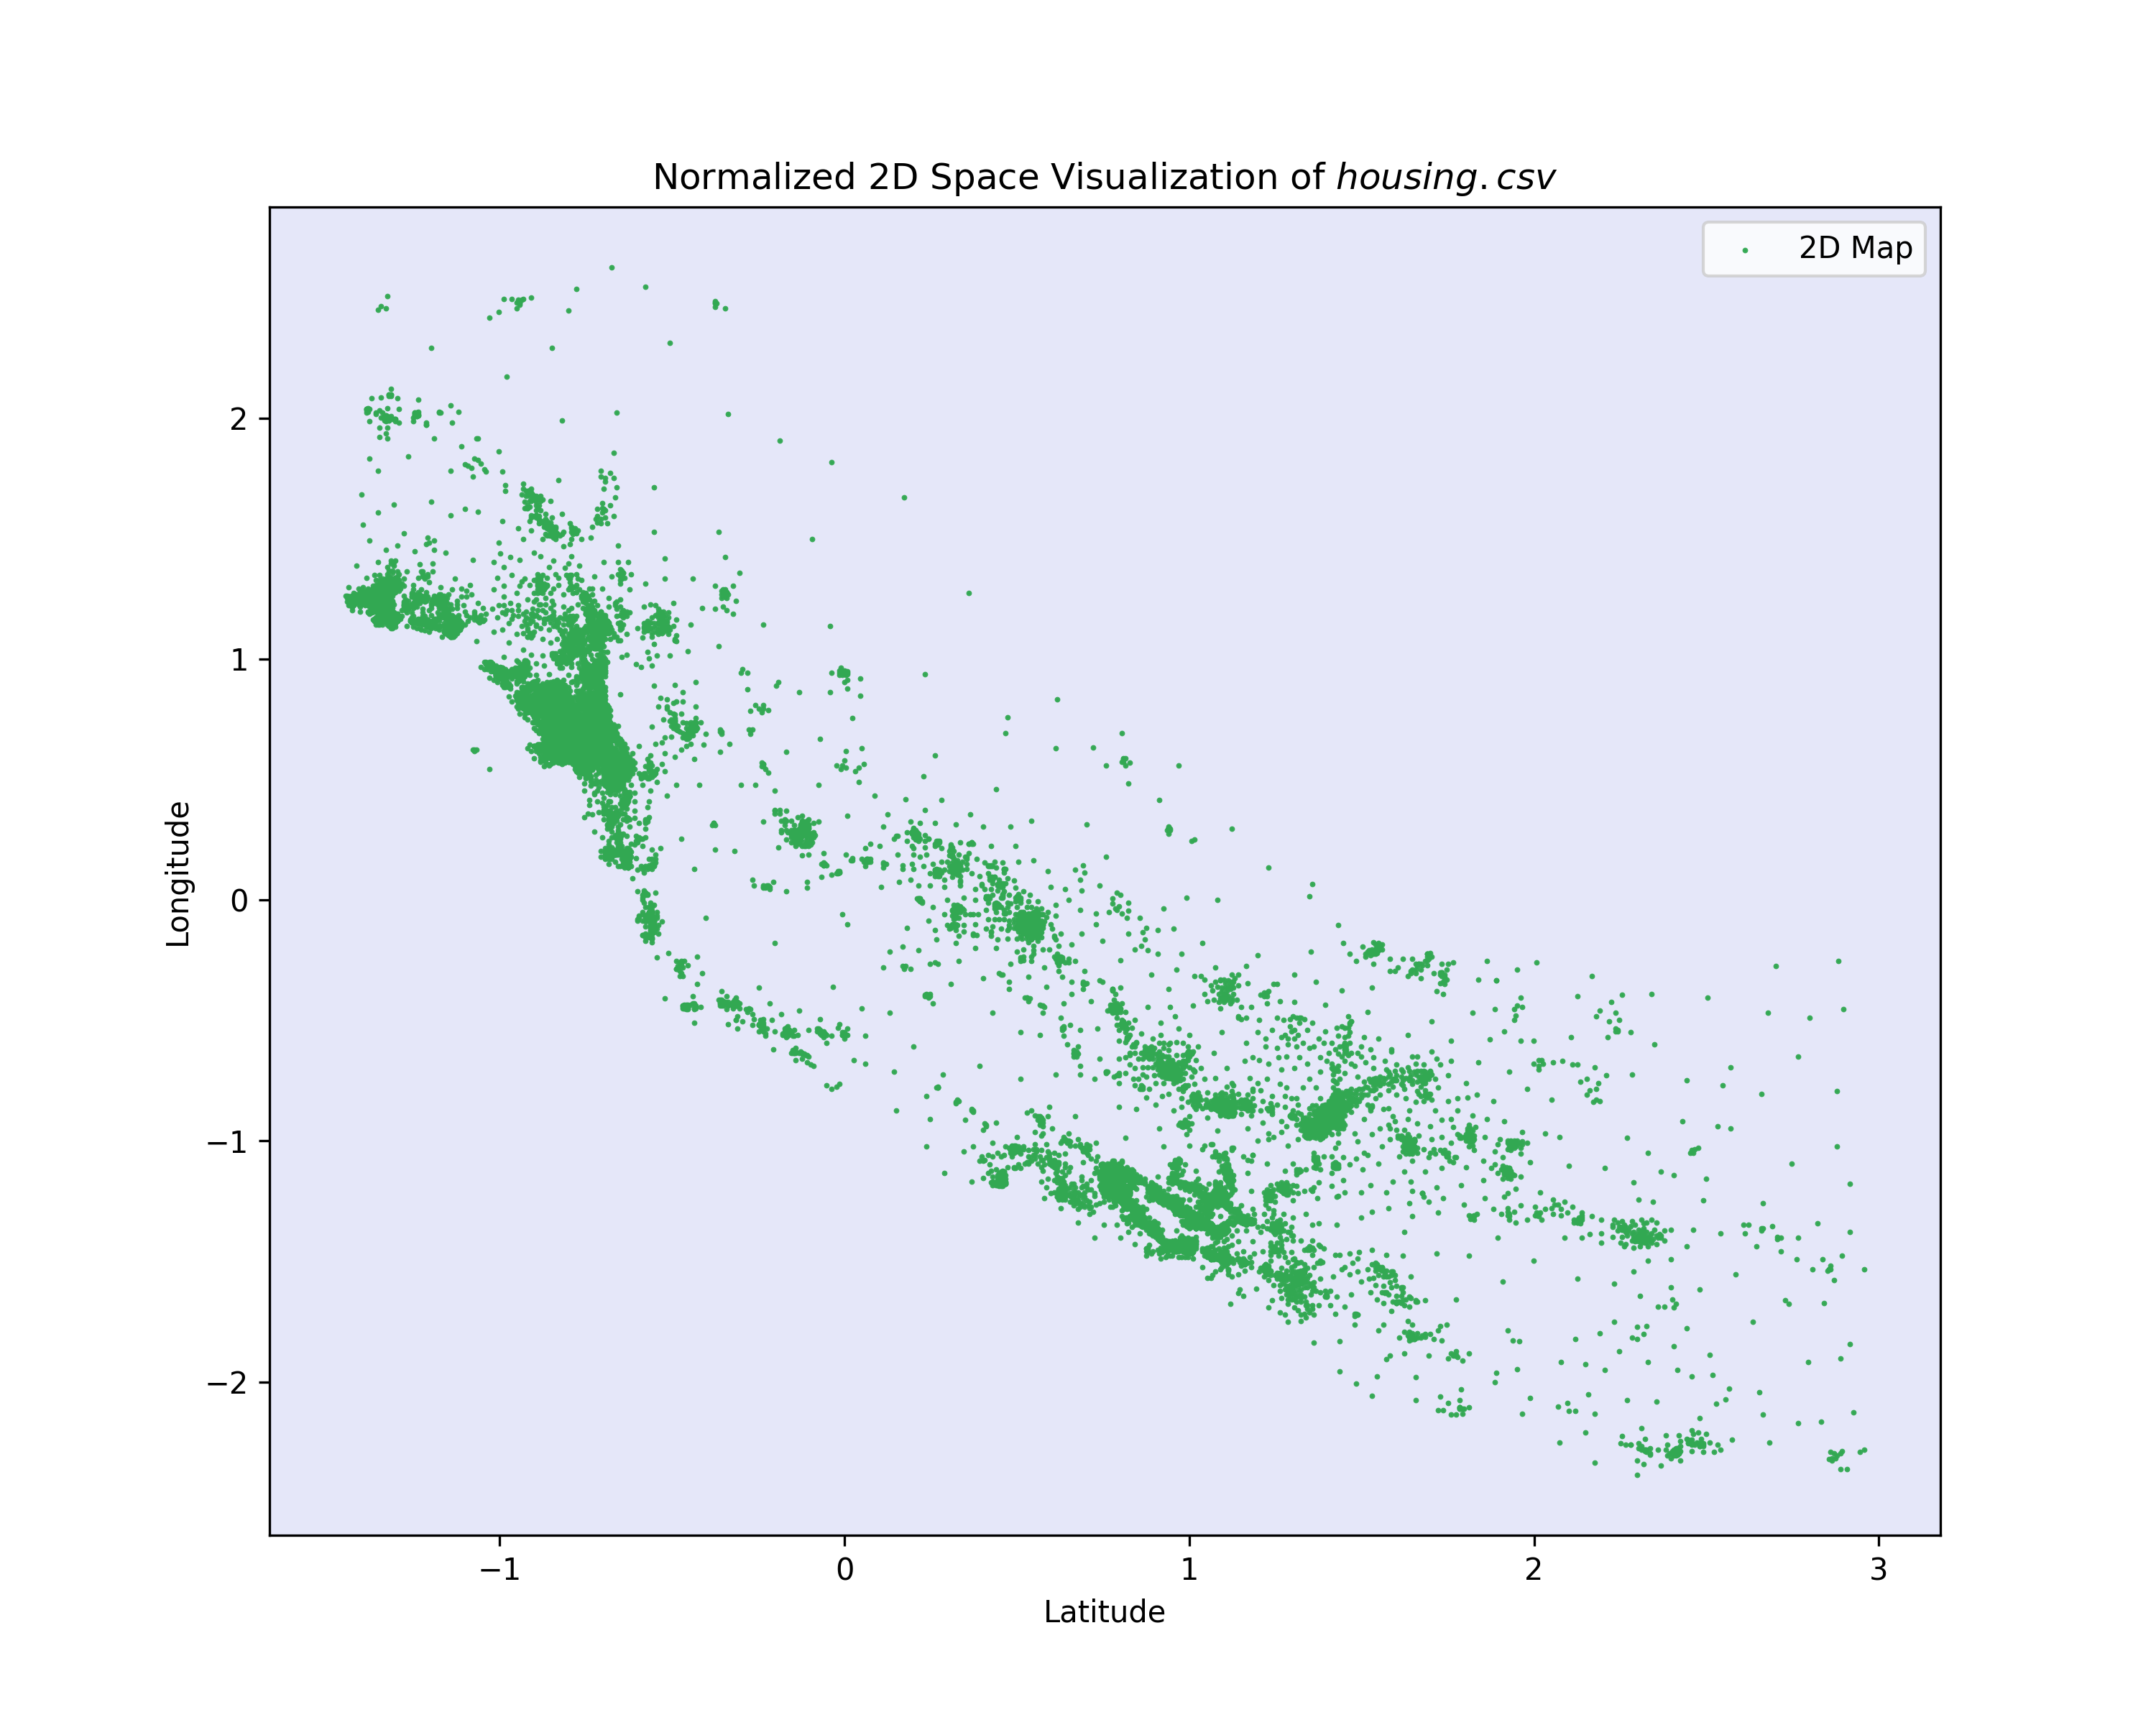
\includegraphics[width=0.75\textwidth]{../plots/q1/2d_housing_scatter.png}
    \centering
    \caption{2D Housing Map - Latitude Longitude Scatterplot}
\end{figure}

% 1.f
\textit{(F)}

\smallskip
Finding the correlation between the input features and \textit{median\_house\_value} we find \textit{median\_income} has a strong positive influence on the value of a home, but for example, \textit{total\_bedrooms} is not as important.

\begin{figure}[!h]
    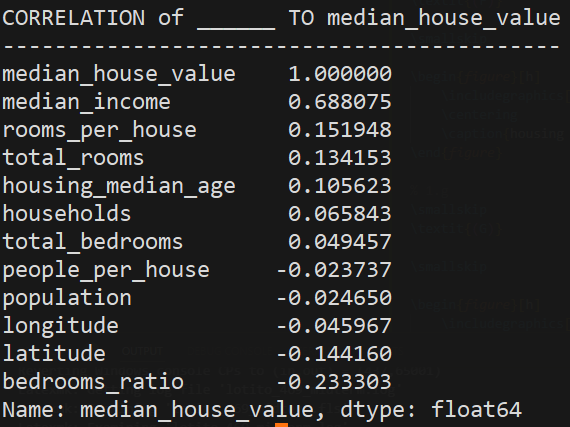
\includegraphics[width=0.45\textwidth]{../logs/housing_corr.png}
    \centering
    \caption{housing Scatter Matrix}
\end{figure}

\clearpage

% 1.g
\smallskip
\textit{(G)}

\smallskip

\begin{figure}[h]
    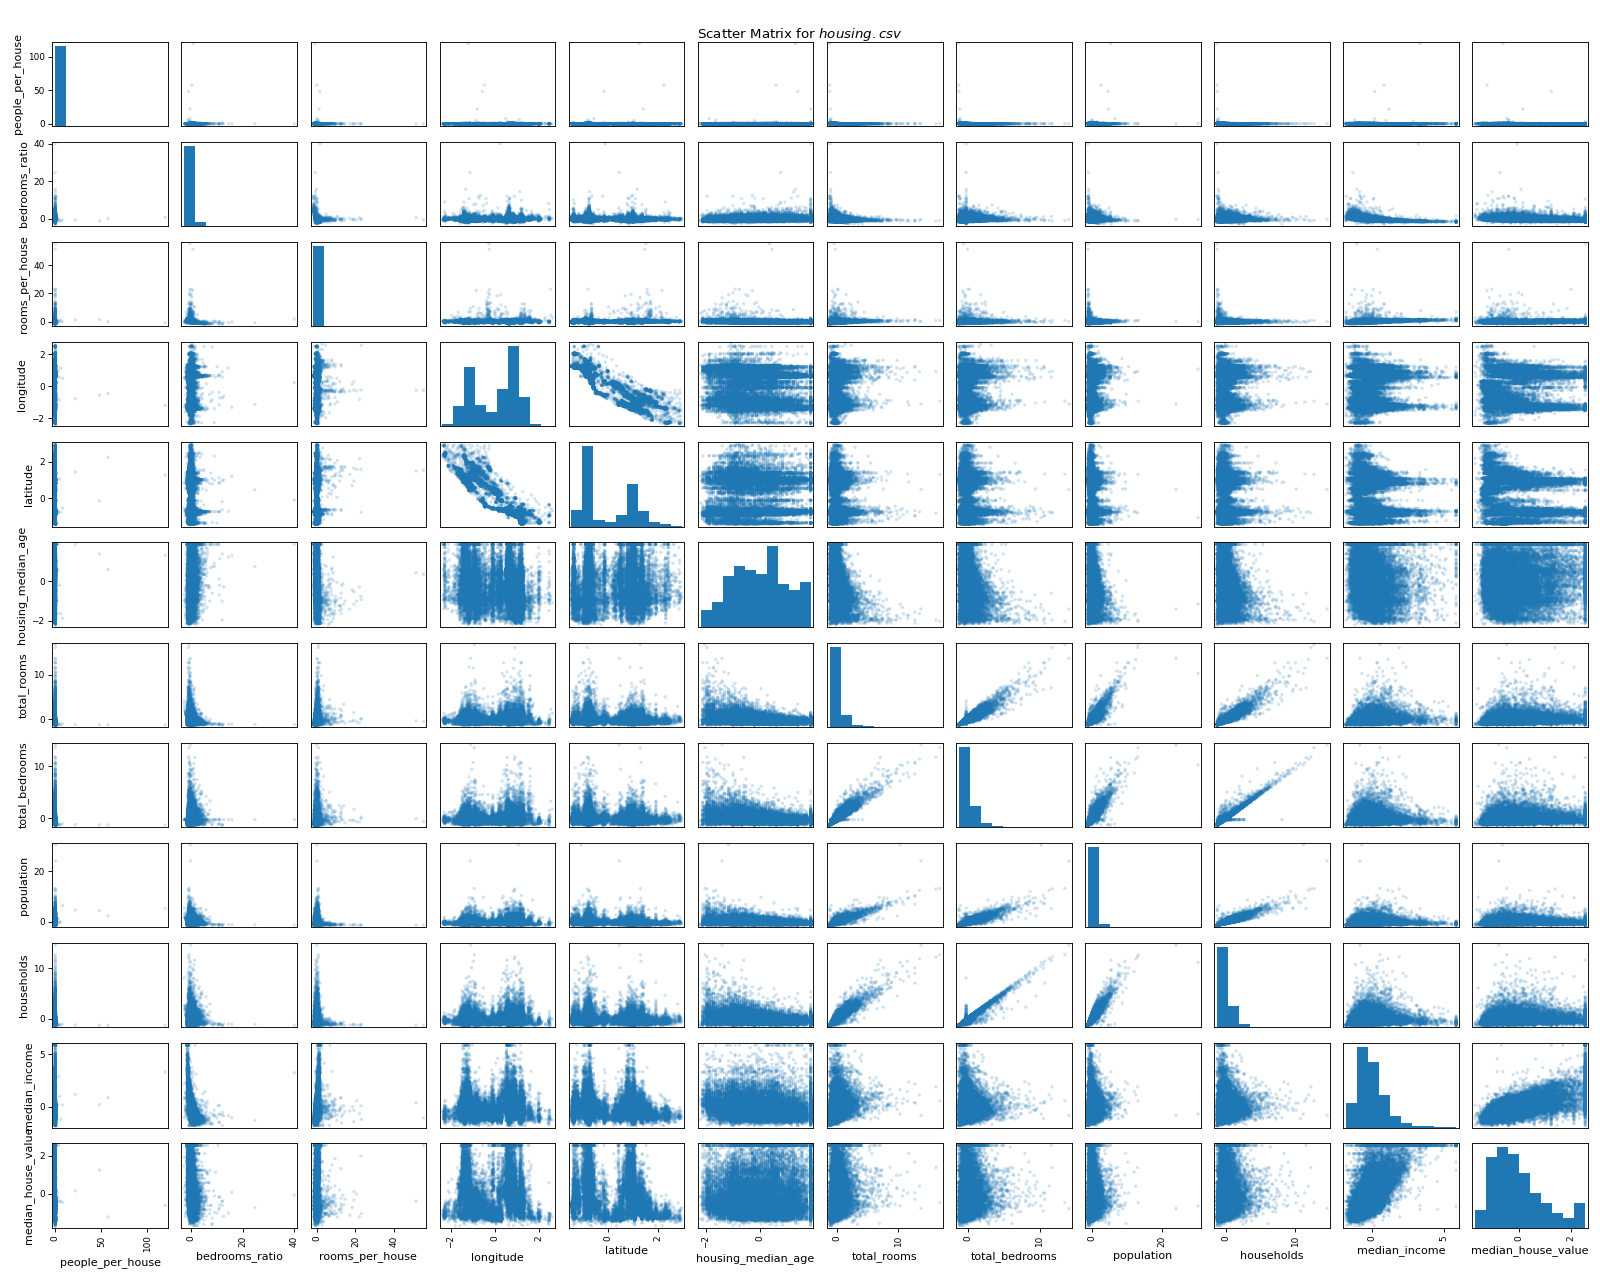
\includegraphics[width=\textwidth]{../plots/q1/housing_scatter_matrix.png}
    \centering
    \caption{housing Scatter Matrix}
\end{figure}


\clearpage

% 1.h
\smallskip
\textit{(H)}

\smallskip 
The derived attributes \textit{rooms per house}, \textit{bedrooms ratio}, and \textit{people per house} are created and inserted as input features in \emph{q1.py} lines 73-88.

% 1.i
\smallskip
\textit{(I)}

\smallskip 
I chose to go the first route, where in lines 62-66, the missing values of \textit{total\_bedrooms}, and the rest of the dataset, were replaced with median values using \textit{SimpleImputer}.

% 1.j
\smallskip
\textit{(J)}

\smallskip
Below, in Fig. \ref{fig:q1_results}, we can see the predictions from our model plotted against the actual target values. Ideally, we would have all predicitions equal to the actual values, and every orange marker would lie along the blue curve. However, the linear model struggles to predict accurately, and we find a spread. 

Also, the \textit{for} loop defined on line 171 trains the linear model for varying sizes of the training set size (almost a kind of cross-validation), where the mean-square-error is calculated for each size (10\%-100\%), and are plotted in Fig. \ref{fig:q1_results}. Here we see testing error falling as the model is trained on larger and larger datasets, but drops off beyond 80\% as the model loses generalization.

It is worth noting that attempting to send the input features of the housing dataset into polynomial space, and then doing a linear regression on that dataset kills any kind of accuracy for any degree other than 1 (1 being nothing changed, still linear).

\begin{figure}[h]
    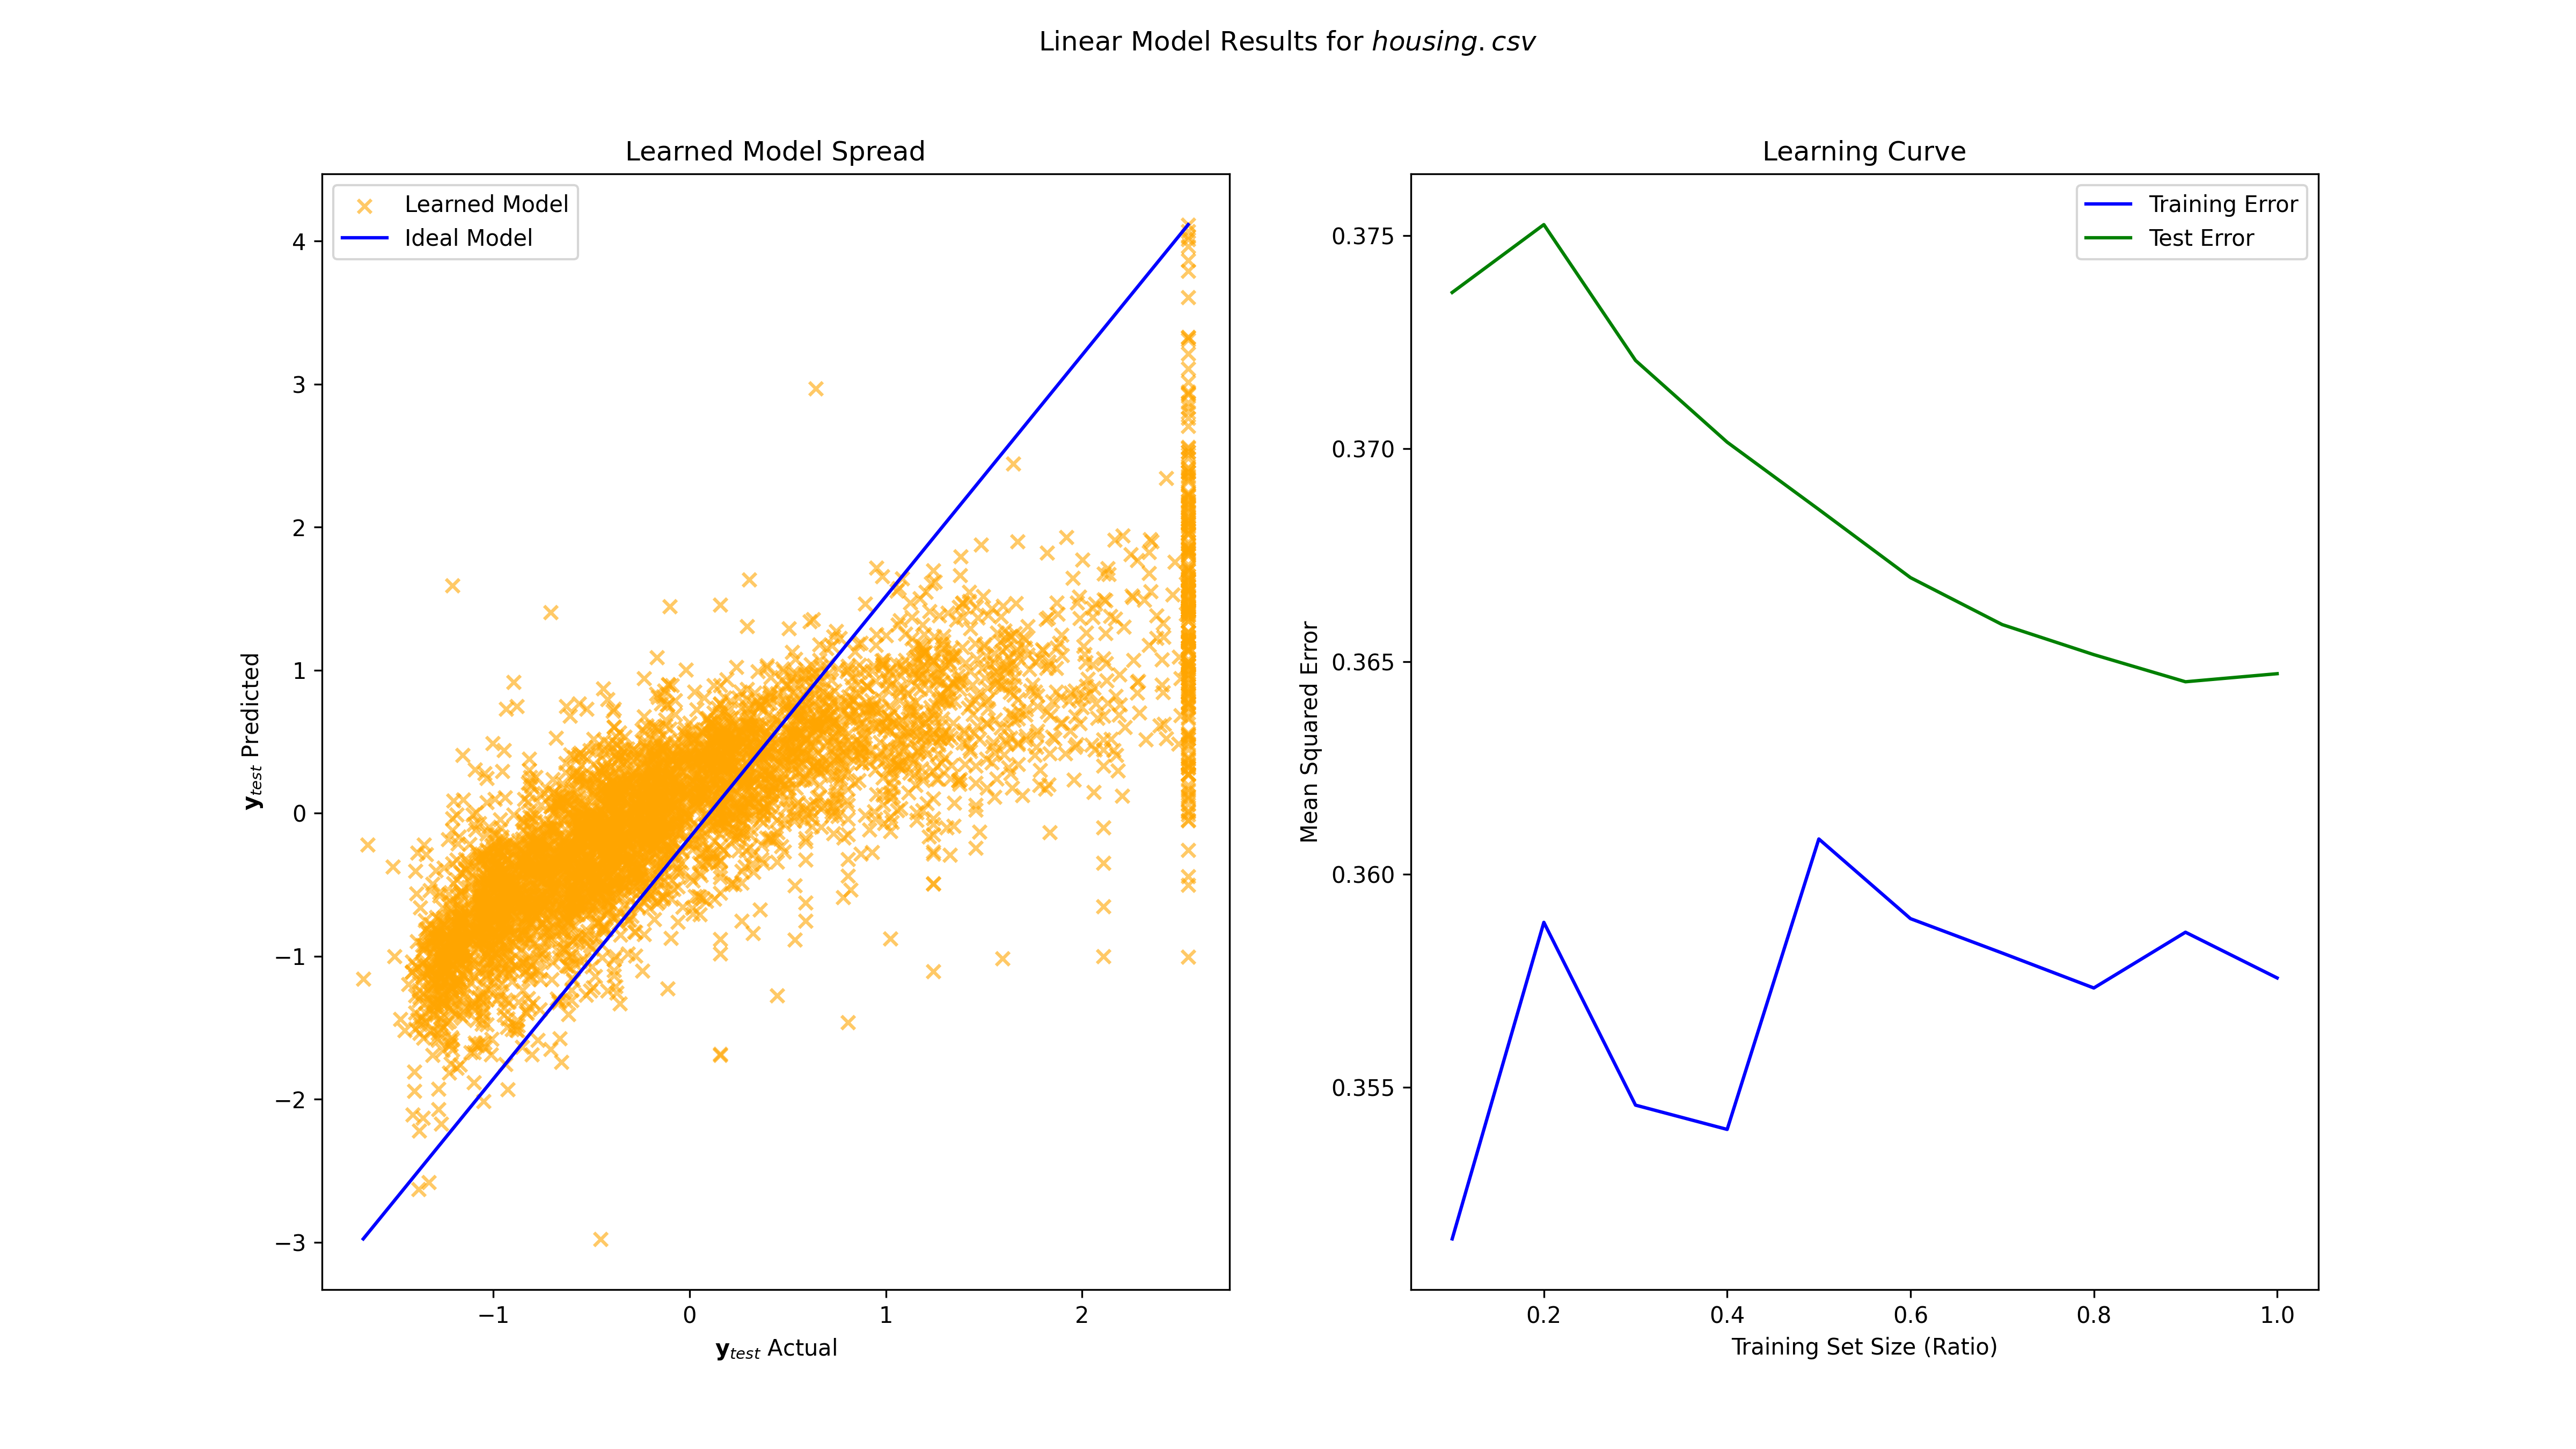
\includegraphics[width=\textwidth]{../plots/q1/linear_model_results.png}
    \centering
    \caption{Linear Model Results: Model Spread (left), Learning Curve (right)}
    \label{fig:q1_results}
\end{figure}

% code for q1
\bigskip
Below is the python code used for Question 1:
\lstinputlisting[caption={File: q1.py}]{../q1.py}

\clearpage

% QUESTION 2
\textbf{Question 2.} \textit{Classification in machine learning.}

\textbf{Solution.}

\smallskip
\textit{(A)}

\smallskip
My best probabilistic classifier has 92.16\% accuracy on the testing set, and my best non-probabilistic classifier has 97.12\% on the testing set. Unfortunately, I was unable to achieve 97\% accuracy for the probabilistic model on the testing set.

\begin{figure}[h]
    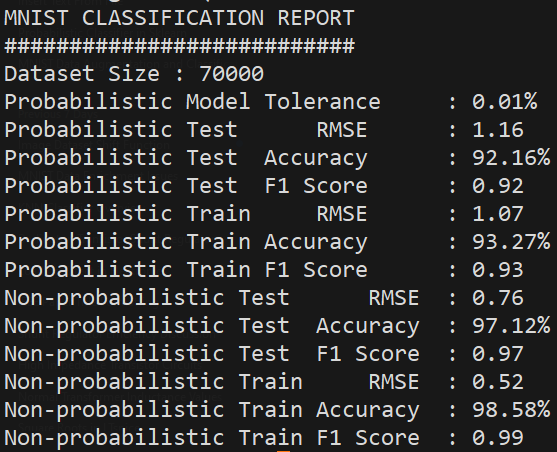
\includegraphics[width=0.45\textwidth]{../logs/mnist.png}
    \centering
    \caption{MNIST Classification Results}
    \label{fig:q2_results}
\end{figure}

\smallskip
\textit{(B)}

I wrote a function called \textit{quad\_direction\_enricher} (lines 43-73) which takes the MNIST dataset and shifts it a user-defined amount of pixels in each of the cardinal directions. The function returns an enriched version of the input features and the corresponding output target, which can then be appended onto the original dataset to increase the amount of data available to train. However, when trained over each of the now 350,000 datapoints, the model drops in accuracy from 92.16\% to 89.97\%. The reason for this I suspect is overfitting, or a reduction in the model's generalization.

\begin{figure}[h]
    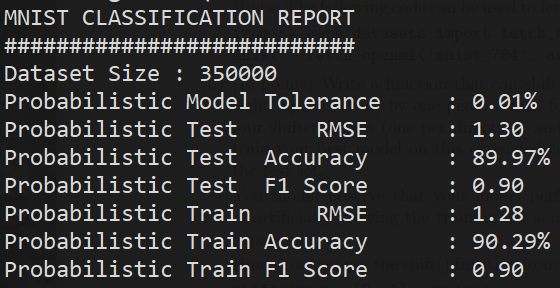
\includegraphics[width=0.45\textwidth]{../logs/mnist_expanded.png}
    \centering
    \caption{Expanded MNIST Classification Results}
    \label{fig:q2_results}
\end{figure}

\smallskip
\textit{(C)}

\smallskip
The non-probabilistic KNN classifier, using 3 neighbors, is in lines 130-155.

\clearpage

\smallskip
\textit{(D)}

\smallskip
No matter what I did, the non-probabilistic KNN classifier always outperformed the probabilistic classifier; for my best model, the non-probabilistic classifier was 4.96\% more accurate than the probabilistic classifier. In terms of computational complexity, the KNN classifier is much more computationally expensive and that is heavily dependent on how many neighbors you wish to use per datapoint, and the computational complexity exponentially increases for the increase in dataset size. For the 350,000 enriched dataset, my computer at 5000MHz could not finish the KNN classifier even after several minutes of waiting. So, there's a trade off. For critical applications that demand accuracy, using the non-probabilistic classifer is best, but for saving compute-power, it is best to choose the probabilistic model.

\begin{figure}[h]
    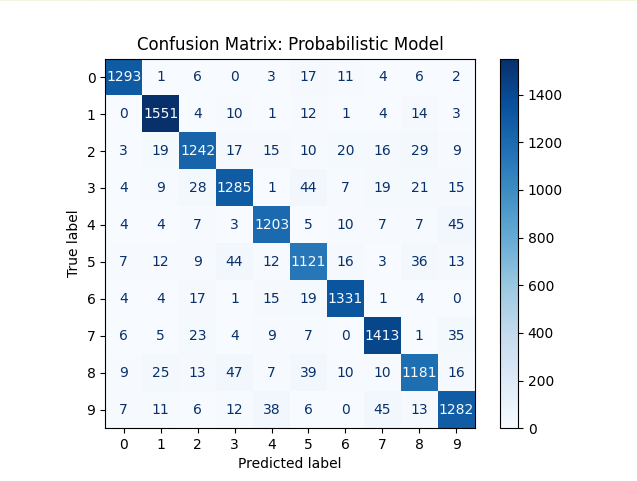
\includegraphics[width=0.6\textwidth]{../plots/q2/prob_confmatrix.png}
    \centering
    \caption{Probabilistic Classifier Confusion Matrix}
    \label{fig:prob_cmatrix}
\end{figure}

\begin{figure}[h]
    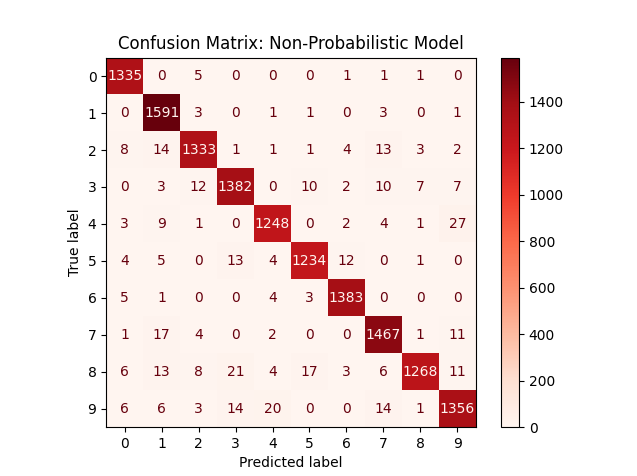
\includegraphics[width=0.6\textwidth]{../plots/q2/nonprob_confmatrix.png}
    \centering
    \caption{Non-probabilistic Classifier Confusion Matrix}
    \label{fig:nonprob_cmatrix}
\end{figure}


% code for q2
\clearpage
Below is the python code used for Question 2:
\lstinputlisting[caption={File: q2.py}]{../q2.py}

\end{document}